\PassOptionsToPackage{hypertexnames=false}{hyperref}
\documentclass[a4paper,fleqn]{cas-sc}

\usepackage[authoryear,longnamesfirst]{natbib}
\usepackage{amsmath,amssymb,amsfonts}
\usepackage{graphicx}
\usepackage{booktabs}
\usepackage{multirow}
\usepackage{algorithm}
\usepackage{algpseudocode}
\usepackage{xurl}

% Anonymous-review placeholders. Replace only after the final author order and
% ORCID records have been approved by all authors.
\RenewDocumentCommand \printorcid {} {}

\newcommand{\breeze}{BREEZE}
\newcommand{\pucond}{N09\_M07\_F10}
% Generated by breeze/scripts/build_paper_tables.py; do not edit.
\newcommand{\BreezePUPassedTests}{12}
\newcommand{\BreezePUHolmBound}{0.001}
\newcommand{\BreezeCWRUPassedTests}{72}
\newcommand{\BreezeCWRURegisteredTests}{72}
\newcommand{\BreezeCWRUAccDeltaMin}{1.7}
\newcommand{\BreezeCWRUAccDeltaMax}{3.5}
\newcommand{\BreezeCWRUFOneDeltaMin}{1.9}
\newcommand{\BreezeCWRUFOneDeltaMax}{3.6}
\newcommand{\BreezeBerkeleyPassedTests}{15}
\newcommand{\BreezeBerkeleyRegisteredTests}{18}
\newcommand{\BreezeBerkeleyUnstructuredPassedTests}{12}
\newcommand{\BreezeBerkeleyUnstructuredRegisteredTests}{12}
\newcommand{\BreezeProposalSlotsPerClass}{150}
\newcommand{\BreezeHealthyAdmissionRate}{60}
\newcommand{\BreezeORAdmissionRate}{60}
\newcommand{\BreezeIRAdmissionRate}{71}
\newcommand{\BreezePULOCOVOneFailures}{57}
\newcommand{\BreezePULOCOVTwoFailures}{60}
\newcommand{\BreezePULOCORegisteredTests}{96}
\newcommand{\BreezeMUTCMPassedTests}{2}
\newcommand{\BreezeMUTCMRegisteredTests}{6}


\begin{document}
\let\WriteBookmarks\relax
\def\floatpagepagefraction{1}
\def\textpagefraction{.001}

\shorttitle{BREEZE physics-verified LLM recipe admission}
\shortauthors{Author One et~al.}

\title[mode=title]{\breeze: Physics-Verified LLM Recipe Generation for
Few-Shot Condition Monitoring}

\author[1]{Author One}
\author[1]{Author Two}

\affiliation[1]{organization={Department},
  city={City},
  country={Country}}

\begin{abstract}
Training a signal generator for every machine and operating regime is often
impractical when labelled faults are scarce. We introduce \breeze, a
training-free generation workflow in which a large language model (LLM)
proposes a structured recipe, a seeded deterministic renderer executes fixed
signal equations, and a verifier admits only candidates satisfying physical
gates calibrated on the real training split. The verifier rejects rather than
repairs a failed waveform, and its pass decision is an auditable
train-calibrated admissibility statement rather than a formal guarantee of
physical validity. On a file-disjoint Paderborn University protocol, LLM
recipes outperform matched rule and random open-loop recipes for Accuracy and
Macro-F1 at 5, 10, and 25 real windows per class; all
\BreezePUPassedTests{} registered comparisons remain significant after Holm
correction ($q<\BreezePUHolmBound$, 20 seeds). On Case Western Reserve
University, all \BreezeCWRUPassedTests{} provenance-valid comparisons across within-load and
held-out loads 1--3 pass Holm correction (40 seeds); the archived held-out-
load0 fold is excluded because it reuses a load0-derived pool. A case/run-
disjoint Berkeley milling test is deliberately qualified:
\BreezeBerkeleyPassedTests/\BreezeBerkeleyRegisteredTests{} comparisons pass,
including all \BreezeBerkeleyUnstructuredPassedTests{} against non-structured baselines, whereas the LLM--rule
advantage is confined to the lower-shot settings. Class-conditional waveform,
envelope, PSD-Wasserstein, band-energy, statistical-distance, and nearest-
neighbour diagnostics provide complementary evidence without being collapsed
into a universal fidelity score. Six predeclared Paderborn cross-condition
attempts fail, establishing the present extrapolation boundary. The results
support LLM-guided, physics-verified admission for the stated few-shot
protocols, not zero-data diagnosis or universal generator superiority.
\end{abstract}

\begin{keywords}
Condition monitoring \sep Large language model \sep Synthetic data \sep
Physics-based verification \sep Few-shot diagnosis \sep Time-series generation
\end{keywords}

\maketitle

\section{Introduction}
\label{sec:intro}

Industrial fault diagnosis is constrained by a structural data problem:
healthy operation is abundant, but labelled faults are scarce, expensive to
seed, and rarely observed under every load and speed. Conventional
augmentation is inexpensive, whereas VAEs, GANs, and diffusion models can
learn richer signal distributions at the cost of target-data training and
model selection~\citep{li2020augmentation,zhao2020vae,zhang2021semivae,
goodfellow2014gan,kingma2014vae,ho2020ddpm}. That cost is justified when a
stable dataset is sufficiently large. It is less attractive when a new
machine, sensor layout, or operating regime provides only a few fault
examples.

LLMs suggest a different design point. Rather than training a waveform
generator, an LLM can propose a compact, machine-conditioned signal recipe.
A numerical renderer then executes the recipe. This separation is useful, but
it does not make the generated waveform reliable. A syntactically valid recipe
can produce unsupported amplitudes, implausible spectral allocation, missing
fault-frequency evidence, or repeated samples. Prompt wording alone cannot
enforce these constraints.

\breeze\ addresses this problem as \emph{admission}. The LLM proposes a JSON
recipe; a fixed renderer maps recipe and seed to a waveform; and a deterministic
verifier, calibrated only from the corresponding outer-training split, decides
whether the candidate may enter the augmentation pool. A rejection report
identifies failed gates and can condition a bounded resampling round. The
verifier does not update the LLM, optimize a target-data generator, inspect the
test split, or alter a rejected waveform. Figure~\ref{fig:framework} summarizes
the resulting closed loop.

\begin{figure*}
  \centering
  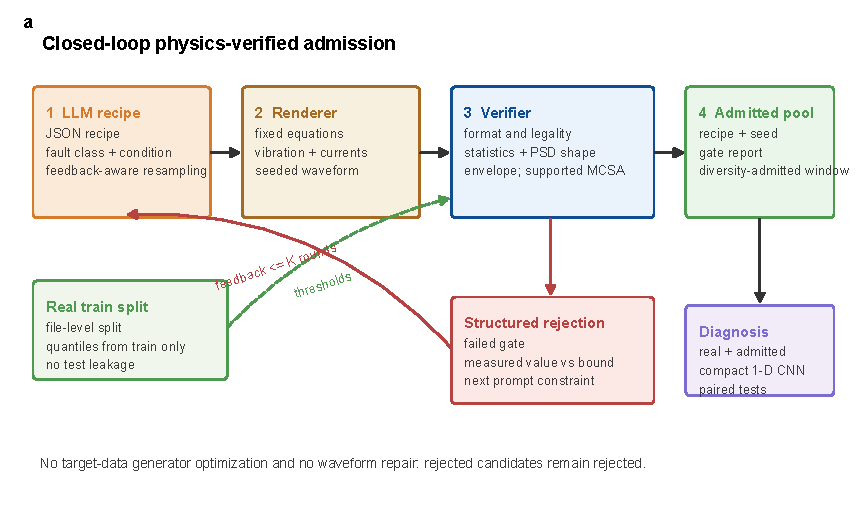
\includegraphics[width=\textwidth]{figs/framework.pdf}
  \caption{The \breeze\ workflow. The LLM proposes a structured recipe, a
  fixed seeded renderer constructs vibration and, when available, current
  channels, and a verifier calibrated exclusively on the real training split
  admits or rejects the candidate. A rejection becomes structured feedback
  for at most $K$ further rounds. Rejected signals are not repaired.}
  \label{fig:framework}
\end{figure*}

The evaluation is organized around three questions. First, does the LLM
contribute beyond a random or engineer-written recipe under an otherwise
matched renderer? Second, do admitted signals exhibit train-supported
time-domain, spectral, envelope, and diversity evidence? Third, does the pool
provide stable diagnostic utility under file-, load-, or experiment-disjoint
few-shot protocols? These questions require paired source ablations,
class-conditional physical diagnostics, leakage-resistant splits, and
corrected statistical tests. A visually plausible trace or a t-SNE map alone
cannot answer them.

The paper makes four contributions:
\begin{enumerate}
  \item It formulates LLM time-series generation as a separable
  recipe--renderer--verifier system, enabling independent auditing of language
  proposals, numerical signal construction, and train-calibrated admission.
  \item It integrates mixed physical gates---format legality, robust signal
  statistics, Welch-PSD shape, envelope-spectrum evidence, reliability-gated
  current evidence, and diversity---into a bounded rejection/resampling loop
  without training a target-data generator.
  \item It establishes the contribution of LLM recipes under matched few-shot
  protocols on three public datasets: PU, CWRU, and Berkeley milling. The
  registered evidence comprises 20 PU seeds and 40 seeds for CWRU and Berkeley,
  with family-wise Holm correction.
  \item It reports negative evidence as part of the method boundary: the full
  six-stage PU leave-one-condition-out (LOCO) failure chain, process-metadata
  confounding in UMich milling, and a stopped MU-TCM inner-validation line.
\end{enumerate}

The supported claim is intentionally narrower than ``LLM signals are
physically correct.'' \breeze\ establishes that admitted candidates satisfy a
declared set of train-supported tests and can improve the stated few-shot
tasks. It does not establish zero-real-data operation, universal
cross-condition morphology transfer, or superiority to every learned
generator.

\section{Related work and positioning}
\label{sec:related}

\subsection{Time-series generation for diagnosis}

General time-series generators include recurrent conditional GANs,
TimeGAN, transformer GANs, variational models, and diffusion
models~\citep{esteban2017rcgan,yoon2019timegan,li2022ttsgan,
li2022ttscgan,liao2020sigcwgan,desai2021timevae,nichol2021improved,
kong2021diffwave,tashiro2021csdi,alcaraz2022sssd,rasul2021timegrad}.
Machinery-specific work has adapted these families to extremely limited or
imbalanced signals. Examples include sparsity-constrained GAN augmentation,
deep feature-enhanced GAN filtering, frequency-learning generation,
spectrum-guided sampling, and FillingGAN~\citep{ma2021scgan,liu2022dfegan,
ko2023flgn,kim2024sgan,lin2025fillinggan}. These systems learn a target signal
distribution; \breeze\ instead studies the operating point where the target
generator is not trained.

\subsection{Physics-informed generation}

Physics-informed learning commonly embeds equations or physical penalties in
a trainable model~\citep{raissi2019pinn}. In rotating machinery, recent GAN and
diffusion systems incorporate impact response, speed modulation, multimodal
features, or condition embeddings~\citep{gao2025physicsgan,
liu2026physicsdiffusion,guo2025diffucd}. Their principal advantage is that the
generator can learn to satisfy the physical objective. Their principal
requirement is retraining and selecting that generator. \breeze\ moves the
physical decision to inference-time admission, which makes it applicable to a
black-box recipe source but also limits what can be concluded from a pass.

Generated-data filtering itself is not new: DFE-GAN and SGAN-DDS already show
that selection and diversity control matter~\citep{liu2022dfegan,kim2024sgan}.
The distinguishing elements here are deterministic train-only calibration,
mixed bearing-diagnostic gates, structured feedback, per-sample audit records,
and explicit separation from waveform repair.

\subsection{LLMs and machinery signals}

LLMs have been reprogrammed for forecasting without task-specific training, used as numerical
forecasters, and supplied with machinery priors for bearing health
management~\citep{jin2024timellm,gruver2023llmtime,peng2025bearllm}. BearGen is
the closest signal-generation study: it uses an LLM to produce signal
descriptions and trains a description-conditioned diffusion generator across
multiple bearing datasets~\citep{lee2026beargen}. \breeze\ differs in both the
LLM output and the optimization boundary. Its LLM emits a structured numerical
recipe, not a waveform or free-text description, and the target-data renderer
has no learned weights.

\begin{table*}[t]
\centering
\caption{Positioning against representative synthetic-signal systems. ``Target
training'' denotes optimization of a generator on the target signal corpus.}
\label{tab:positioning}
\small
\setlength{\tabcolsep}{4pt}
\begin{tabular}{@{}p{2.2cm}p{3.0cm}p{1.8cm}p{2.3cm}p{4.0cm}@{}}
\toprule
Method family & Generative mechanism & Target training & Physical control & Primary evidence pattern \\
\midrule
DFE-GAN / SGAN-DDS & Learned adversarial generator plus filtering or sampling & Yes & Learned features and spectrum guidance & Fidelity, diversity, and diagnosis \\
Physics-informed GAN / diffusion & Learned generator with physical priors or condition embedding & Yes & Training loss or architecture & Mechanism, multidomain fidelity, diagnosis \\
BearGen & LLM descriptions condition a learned diffusion model & Yes & Description guidance and learned denoising & Eight bearing datasets, quality, few-shot, cost \\
\breeze & LLM JSON recipe plus fixed seeded renderer & No & Train-calibrated admission and rejection & Source ablation, gate reports, physical distances, paired diagnosis \\
\bottomrule
\end{tabular}
\end{table*}

\subsection{Diagnostic observables used as gates}

Rolling-element faults excite resonances through stochastic or
pseudo-cyclostationary impacts. Envelope analysis, spectral kurtosis, and the
fast kurtogram are established ways to expose these signatures
\citep{randall2011bearing,antoni2006spectral,antoni2007kurtogram}. Welch PSD
estimation provides a stable spectral-shape representation
\citep{welch1967psd}. Motor-current sidebands can provide complementary bearing
evidence when the real training data support separability~\citep{schoen1995mcsa}.
\breeze\ uses these quantities as measurable admission evidence, not as a
complete simulator of bearing dynamics.

\section{Problem formulation and framework}
\label{sec:method}

\subsection{Train-calibrated admission}

Let $\mathcal{D}_{\mathrm{tr}}=\{(x_i,y_i,m_i)\}_{i=1}^{n}$ denote real
training windows, class labels, and available machine metadata. For requested
class $y$ and condition $m$, the LLM proposes recipe $r_t$ at feedback round
$t$. A seeded renderer $R$ produces
\begin{equation}
  \tilde{x}_{t,s}=R(r_t,m;s),
\end{equation}
where $s$ is archived with the recipe. A verifier $V$ returns an admission
indicator and a report,
\begin{equation}
 (a_{t,s},q_{t,s})=V(\tilde{x}_{t,s},y,m;\mathcal{D}_{\mathrm{tr}}),
 \qquad a_{t,s}\in\{0,1\}.
 \label{eq:verifier}
\end{equation}
No test sample contributes to $R$, gate calibration, feedback, or pool
selection.

The gate family is mixed. It cannot be represented correctly by one generic
one-sided inequality. For deterministic feature $f_j$, class-supported bounds
$[l_{j,y,m},u_{j,y,m}]$, healthy fault-prominence score $p_f$, physical
embedding $e(x)$, and current admitted set $\mathcal{S}_y$, the active rules are
\begin{align}
 l_{j,y,m}\leq f_j(x)\leq u_{j,y,m} &\quad\text{(interval)},\nonumber\\
 f_j(x)\leq u_{j,y,m}\ \text{or}\ f_j(x)\geq l_{j,y,m}
   &\quad\text{(one-sided evidence)},\nonumber\\
 p_f(x)\leq u_{f,\mathrm{healthy}}
   &\quad\text{(healthy suppression)},\nonumber\\
 \min_{z\in\mathcal{S}_y}\lVert e(x)-e(z)\rVert_2\geq\delta_y
   &\quad\text{(diversity)}.
 \label{eq:mixed-gates}
\end{align}
The admissible set is the intersection of the active predicates. Membership
states only that the configured gates passed under their training calibration.

\subsection{Responsibility boundaries}

Figure~\ref{fig:boundary} separates four responsibilities. The LLM selects
recipe fields; the renderer enforces the stated signal equations; the verifier
measures compatibility with train-supported evidence; and the downstream
classifier measures utility. This separation prevents the verifier's
contribution from being attributed to intrinsic LLM knowledge.

\begin{figure*}
  \centering
  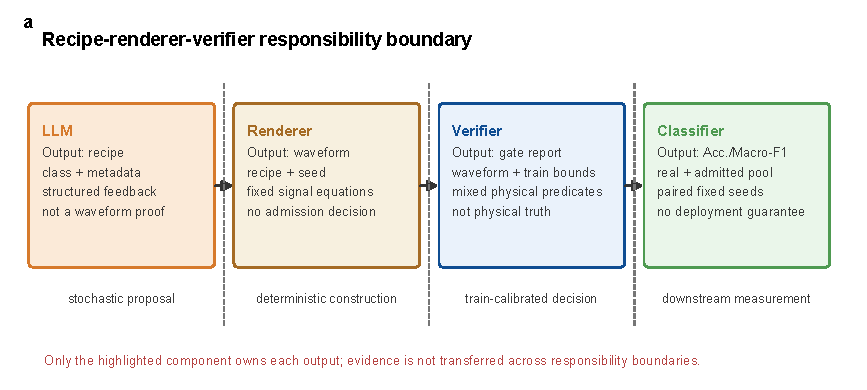
\includegraphics[width=\textwidth]{figs/responsibility_boundary.pdf}
  \caption{Component responsibility boundary. The LLM selects recipe
  parameters; the renderer alone constructs waveforms; the verifier admits or
  rejects without repair; and the classifier is used only for downstream
  evaluation. Every formal source comparison holds renderer and classifier
  fixed.}
  \label{fig:boundary}
\end{figure*}

The recipe records shaft and fault frequencies, target RMS, periodic-impact
rate, amplitude, decay, resonance, slip jitter, amplitude variation,
load-zone modulation, background components, random machine transients,
eight vibration-band weights, and optional two-phase current parameters. The
initial prompt supplies class, condition metadata, bearing kinematics, a
training-derived exemplar description, and the JSON schema. A feedback prompt
adds the previous recipe and each failed gate's measured value and supported
bound, and requests a proportional parameter change. Complete prompt builders
and schemas are preserved in \texttt{src/llm.py}.

\subsection{Seeded renderer}

For PU vibration, the renderer combines deterministic background harmonics,
Poisson machine transients, a jittered train of resonant impacts, and
band-shaped noise:
\begin{align}
x_v(t)={}&\sum_q A_q\sin(2\pi f_qt+\phi_q)
 +\sum_{\ell} b_{\ell}h(t-u_{\ell})
 +\sum_k a_kh(t-t_k)+\epsilon_b(t),\label{eq:vibration}\\
h(\tau)={}&\mathbf{1}_{\tau\geq0}\exp(-\tau/\tau_d)
             \sin(2\pi f_r\tau+\phi),\label{eq:impact}\\
t_{k+1}-t_k={}&f_f^{-1}(1+\xi_k).
\end{align}
Here $u_\ell$ follows a Poisson background process, $f_f$ is the requested
fault frequency, and $\xi_k$ is bounded recipe jitter. Inner-race impact
amplitudes may be modulated at shaft frequency. The renderer shapes additive
noise over the fixed eight-band grid and applies the same deterministic target-
RMS normalization to every recipe source before verification. These operations
are part of $R$; they are not repairs applied after a gate decision.

When two phase currents are available, channel $p$ is rendered as
\begin{align}
i_p(t)={}&A_p\bigl[1+\beta\cos(2\pi f_ft+\psi)\bigr]
\left[\sin(2\pi f_et+\phi_p)
+\sum_{h\in\{3,5,7\}}\rho_h\sin(2\pi hf_et+\phi_{p,h})\right]
+\eta_p(t),
\label{eq:current}
\end{align}
where $f_e$ is supply frequency. The code and archived seed make $R(r,m;s)$
deterministic.

Berkeley uses the same responsibility principle but not bearing kinematics.
Its multichannel renderer starts from a train-only channel exemplar, adds the
recipe's transient and band-energy structure, and preserves channel-specific
location and scale. This is a milling renderer calibrated inside the outer
training fold; it is not presented as the same physical model as
Eqs.~\eqref{eq:vibration}--\eqref{eq:current}.

\subsection{Verifier gates}

The verifier evaluates the following active evidence:
\begin{enumerate}
  \item \textbf{Legality:} exact shape, finite samples, non-degenerate
  channels, and absence of long repeated runs.
  \item \textbf{Robust statistics:} class- and channel-conditional RMS,
  standard deviation, peak, kurtosis, skewness, and crest factor inside
  train-derived quantile or robust-union domains.
  \item \textbf{Spectral shape:} triangular-band Welch-PSD fractions and
  PSD-CDF Wasserstein-1 distance to the class training reference.
  \item \textbf{Envelope evidence:} resonance-band Hilbert demodulation,
  prominence near the requested BPFO, BPFI, BSF, or FTF frequency, harmonic support,
  and suppression of unsupported peaks for healthy candidates.
  \item \textbf{Current evidence:} vector-current sideband scores when, and
  only when, training data establish class separability. Otherwise the score
  is logged but is not a hard constraint.
  \item \textbf{Diversity:} a lower nearest-neighbour bound in the physical
  feature embedding relative to a train-derived real--real reference.
\end{enumerate}
The reliability condition on current evidence is important: PU does not
support a universal hard MCSA constraint, so current-signature consistency is
not claimed for every admitted pool.

\subsection{Closed-loop construction and audit records}

\begin{algorithm}[t]
\caption{\breeze\ recipe admission for one proposal slot}
\label{alg:loop}
\begin{algorithmic}[1]
\Require class $y$, condition $m$, LLM $G$, renderer $R$, verifier $V$,
round limit $K$, renderer seeds $\mathcal{S}$
\State $q_{-1}\gets\varnothing$
\For{$t=0$ to $K$}
  \State $r_t\gets G(y,m,q_{t-1})$
  \ForAll{$s\in\mathcal{S}$}
    \State $\tilde{x}_{t,s}\gets R(r_t,m;s)$
    \State $(a_{t,s},q_{t,s})\gets V(\tilde{x}_{t,s},y,m)$
    \If{$a_{t,s}=1$}
      \State archive recipe, seed, waveform hash, and full gate report
      \State \Return admitted slot and all diversity-admitted windows
    \EndIf
  \EndFor
  \State $q_t\gets\mathrm{AggregateFailures}(\{q_{t,s}\})$
\EndFor
\State \Return rejected slot with terminal failure report
\end{algorithmic}
\end{algorithm}

A \emph{slot} is one requested class-conditioned recipe unit. A slot can
archive several round candidates, and an admitted recipe can be rendered with
several deterministic seeds; therefore one admitted slot can yield more than
one window. A \emph{window} is the actual $C\times N$ tensor supplied to the
classifier. Slot counts measure LLM proposal cost; window counts measure the
augmentation budget. The frozen pipeline renders three seeds per recipe and
can retain additional diversity-admitted expansions, so these units must not
be interchanged.

The CWRU archive records the OpenAI-compatible model identifier
\texttt{mimo-v2.5}, temperature 0.8, top-$p$ 0.9, and maximum 900 output
tokens. Provider-side sampling seeds were not exposed. The earlier PU archive
preserves prompts, recipes, rendered pools, and local seeds, but its exact
provider version and top-$p$ are absent from the original provenance record.
Consequently, the frozen PU pools are reproducible from archived recipes and
renderer seeds, while identical regeneration of the original language
responses is not claimed. No new LLM call was made during manuscript assembly.

\section{Experimental design}
\label{sec:setup}

\subsection{Public datasets and leakage-resistant splits}

Table~\ref{tab:datasets} summarizes the three formal public datasets. PU and
CWRU are established bearing benchmarks~\citep{lessmeier2016pu,
smith2015cwru}; Berkeley milling is distributed through the NASA prognostics
repository~\citep{agogino2007milling}. Splits are formed by file, load, or
case/run before window sampling. No window-random result is used in the formal
claims.

\begin{table*}[t]
\centering
\caption{Formal datasets and frozen protocols. Counts are windows after the
declared split.}
\label{tab:datasets}
\small
\setlength{\tabcolsep}{4pt}
\begin{tabular}{@{}p{1.4cm}p{2.0cm}p{2.2cm}p{2.8cm}p{1.7cm}p{3.5cm}@{}}
\toprule
Dataset & Sampling and input & Classes & Operating regime & Train/test & Split unit \\
\midrule
PU & 8 kHz, 3 channels, 2048 samples & healthy, OR, IR & \pucond: 900 rpm, 0.7 Nm, 1000 N & 3846/962 & chronological measurement files within bearing; zero shared file/window keys \\
CWRU & 12 kHz drive-end vibration, 2048 samples & healthy, IR, ball, OR & motor loads 0--3; defects 0.007--0.028 in & 696/306 for within-load0 & chronological within-file for load0; loads 1--3 held out separately for clean transfer tests \\
Berkeley & 250 Hz, 6 channels, 512 samples & healthy ($VB<0.2$), degraded ($VB\geq0.2$) & feed, depth, and material combinations & 1836/646 & disjoint machining case/run groups \\
\bottomrule
\end{tabular}
\end{table*}

The PU file split contains training counts 1200/1202/1444 and test counts
300/301/361 for healthy/OR/IR. The retained channels are one vibration and two
phase-current channels. CWRU evaluates a within-load0 split and three clean
transfer folds in which load1, load2, or load3 is held out. The frozen
synthetic pools were derived from load0, which belongs to the training side of
these three folds. The archived held-out-load0 fold is retained only as an
audit artifact because reusing those pools gives it target-load provenance.
Berkeley channels are spindle AC and DC current, table and
spindle vibration, and table and spindle acoustic emission. Its healthy/
degraded threshold and split were frozen after train-only inner validation and
before the one-time 40-seed formal run.

\subsection{Recipe-source and augmentation controls}

The central ablation changes the recipe source while retaining the applicable
renderer, data split, synthetic budget, CNN, and paired seeds:
\begin{itemize}
  \item \textbf{LLM + verifier:} class- and condition-aware JSON recipe,
  physical admission, and bounded feedback.
  \item \textbf{Rule + verifier:} engineer-written class template with
  train-supported parameter ranges, the same renderer, and the same verifier;
  no LLM call.
  \item \textbf{Random open-loop:} random legal recipe values rendered without
  feedback. On PU this is the matched non-semantic downstream control; a
  separate random-recipe verifier audit is also reported.
  \item \textbf{Noise augmentation:} real few-shot windows with channel-scaled
  jitter and amplitude scaling, using the same synthetic count.
  \item \textbf{Real only:} the paired few-shot subset without synthetic data.
\end{itemize}
The formal CWRU family contains LLM comparisons with rule, noise, and real
only over within-load0 and held-out loads 1--3. Berkeley additionally contains
random open-loop. PU Phase-A focuses on
the sharper recipe-source question: LLM versus rule and random open-loop.

TimeGAN and 1-D DDPM were implemented with checkpointed full-fold and few-shot
training, but their archived runs are smoke/development outputs rather than a
completed predeclared formal baseline. They are therefore excluded from every
quantitative claim. The paper does not claim superiority to trained GAN or
diffusion methods until a matched formal run exists. FID/KID-style learned
distances are likewise not reported because no validated domain feature
extractor was fixed; their general role is described by
\citet{heusel2017fid,binkowski2018mmdgan}.

\subsection{Few-shot classifier and statistical protocol}

All methods within a dataset share the same compact 1-D CNN: three convolution
blocks with 16, 32, and 64 channels, kernels 15, 9, and 5, stride two,
max-pooling after the first two blocks, adaptive average pooling to length
eight, and a linear classifier. Adam uses learning rate $3\times10^{-4}$,
weight decay $10^{-4}$, batch size 32, and cross-entropy loss. PU uses 60
epochs; the frozen CWRU and Berkeley protocols use 20. Training-channel mean
and standard deviation normalize both train and test data.

PU uses $n_{\mathrm{real}}\in\{5,10,25\}$, 150 synthetic windows per class,
and 20 paired seeds. CWRU uses the same shot counts, 20 synthetic windows per
class, and 40 seeds. Berkeley uses $n_{\mathrm{real}}\in\{2,5,10\}$, 20
synthetic windows per class, and 40 seeds. Accuracy and Macro-F1 are primary.
The seed selects the same real subset and classifier initialization for every
method in its paired cell.

Registered one-sided Wilcoxon signed-rank tests compare paired seeds
\citep{wilcoxon1945paired}. Holm correction controls family-wise error within
each predeclared comparison family~\citep{holm1979multiple}. Benjamini--
Hochberg values were retained only as secondary audit output, not substituted
for the registered Holm decision~\citep{benjamini1995fdr}. We report direction,
adjusted decision, seed count, and the complete pass pattern; an unadjusted
$p$ value near 0.05 is not called significant.

\subsection{Physical and distribution diagnostics}

Diagnostics are computed class by class against the outer-training reference:
RMS, kurtosis, skewness, crest factor, peak value, BPFO/BPFI/BSF/FTF peak
alignment where applicable, envelope prominence and harmonic support,
PSD-CDF Wasserstein-1 distance, relative band-energy error, and nearest-
neighbour distance. Wasserstein distance follows the optimal-transport
interpretation of \citet{villani2009transport}. MMD is retained in the
archived feature audit using an RBF kernel and the median pairwise-distance
bandwidth~\citep{gretton2012mmd}; the main figure reports directly interpretable
distances. No t-SNE or UMAP plot is used as core evidence. Mixup is discussed
as a conventional augmentation family but is not part of the frozen formal
comparison~\citep{zhang2018mixup}.

\section{Results}
\label{sec:results}

\subsection{LLM recipe contribution on PU}

Table~\ref{tab:pu-phasea} answers the primary source-ablation question. LLM
recipes exceed rule and random open-loop recipes at every shot count for both
metrics. All \BreezePUPassedTests{} registered pairwise tests remain
significant after Holm correction ($q<\BreezePUHolmBound$).
Table~\ref{tab:pu-phasea} reports the paired protocol means and standard
deviations.

% Generated by breeze/scripts/build_paper_tables.py; do not edit.
\begin{table}[t]
\centering
\caption{PU Phase-A v2 file-split results (20 seeds; $n_{\rm syn}=150$ per class). Holm $q$ values test LLM $K=3$ superiority within each registered family.}
\label{tab:pu-phasea}
\small
\begin{tabular}{rrccccc}
\toprule
$n_{\rm real}$ & metric & LLM $K=3$ & rule & random & $q_{\rm rule}$ & $q_{\rm random}$ \\
\midrule
5 & Acc. & 0.777 $\pm$ 0.027 & 0.696 $\pm$ 0.053 & 0.450 $\pm$ 0.029 & <0.001 & <0.001 \\
5 & Macro-F1 & 0.776 $\pm$ 0.026 & 0.691 $\pm$ 0.049 & 0.436 $\pm$ 0.053 & <0.001 & <0.001 \\
10 & Acc. & 0.796 $\pm$ 0.030 & 0.724 $\pm$ 0.042 & 0.483 $\pm$ 0.013 & <0.001 & <0.001 \\
10 & Macro-F1 & 0.800 $\pm$ 0.029 & 0.724 $\pm$ 0.040 & 0.488 $\pm$ 0.015 & <0.001 & <0.001 \\
25 & Acc. & 0.818 $\pm$ 0.021 & 0.769 $\pm$ 0.025 & 0.529 $\pm$ 0.022 & <0.001 & <0.001 \\
25 & Macro-F1 & 0.821 $\pm$ 0.022 & 0.770 $\pm$ 0.024 & 0.527 $\pm$ 0.017 & <0.001 & <0.001 \\
\bottomrule
\end{tabular}
\end{table}


Figure~\ref{fig:downstream} shows paired seed-level deltas rather than only
means. The PU LLM advantage is positive for both Accuracy and Macro-F1 across
all registered source comparisons. This establishes an LLM contribution under
the frozen renderer and protocol; it does not establish that the LLM alone
created the physical evidence, because renderer and verifier remain necessary
parts of the system.

\begin{figure*}
  \centering
  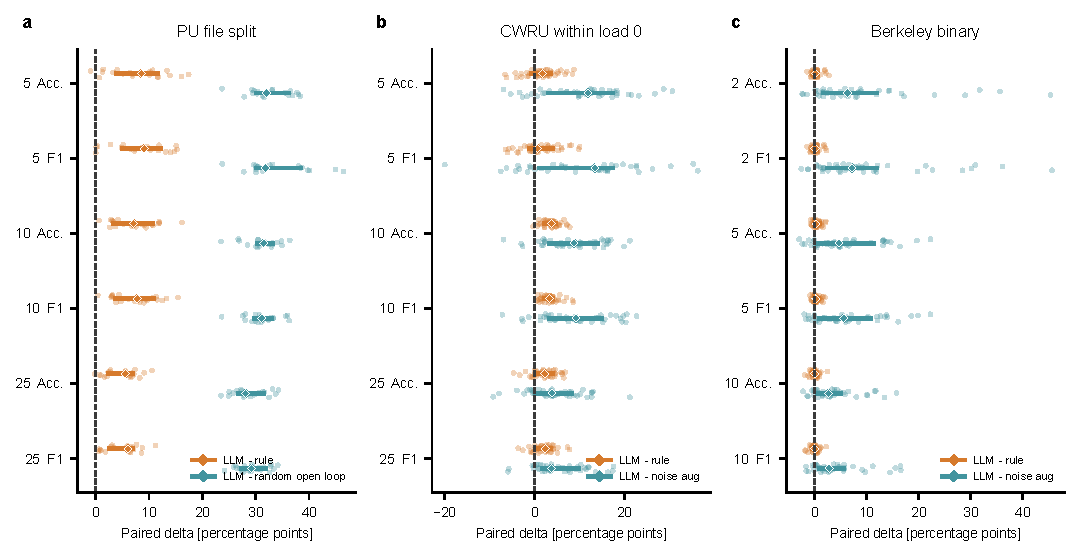
\includegraphics[width=\textwidth]{figs/downstream_bars.pdf}
  \caption{Paired downstream deltas. Points are seed-level differences; thick
  segments show interquartile ranges and diamonds show medians. (a) PU LLM
  minus rule or random open-loop. (b) CWRU within-load0 LLM minus rule or noise
  augmentation. (c) Berkeley LLM minus rule or noise augmentation. The dashed
  line is zero.}
  \label{fig:downstream}
\end{figure*}

\subsection{CWRU within-load and leave-one-load-out}

CWRU extends the evidence across four motor loads and four fault classes.
Within load0, LLM recipes outperform rule and noise augmentation at every shown
shot count (Table~\ref{tab:cwru}). Across that split and the three provenance-
valid transfer folds,
\BreezeCWRUPassedTests/\BreezeCWRURegisteredTests{} registered
LLM-comparator tests have positive direction and pass Holm correction.
Figure~\ref{fig:cross} reports LLM--rule
deltas when the source load0 pool is transferred to held-out loads 1--3:
Accuracy improvements range from \BreezeCWRUAccDeltaMin{} to
\BreezeCWRUAccDeltaMax{} percentage points, and Macro-F1 improvements from
\BreezeCWRUFOneDeltaMin{} to \BreezeCWRUFOneDeltaMax{} points across shots
and folds.

% Generated by breeze/scripts/build_paper_tables.py; do not edit.
\begin{table}[t]
\centering
\caption{CWRU within-load0 results (40 seeds). All 90/90 registered LLM-comparator tests across within and four LOLO folds pass Holm correction; the table gives the within-load0 means.}
\label{tab:cwru}
\small
\begin{tabular}{rrccc}
\toprule
$n_{\rm real}$ & metric & LLM & rule & noise augmentation \\
\midrule
5 & Acc. & 0.564 $\pm$ 0.068 & 0.549 $\pm$ 0.053 & 0.454 $\pm$ 0.066 \\
5 & Macro-F1 & 0.567 $\pm$ 0.075 & 0.554 $\pm$ 0.062 & 0.460 $\pm$ 0.084 \\
10 & Acc. & 0.621 $\pm$ 0.037 & 0.584 $\pm$ 0.033 & 0.534 $\pm$ 0.065 \\
10 & Macro-F1 & 0.646 $\pm$ 0.050 & 0.611 $\pm$ 0.046 & 0.554 $\pm$ 0.082 \\
25 & Acc. & 0.674 $\pm$ 0.037 & 0.652 $\pm$ 0.037 & 0.628 $\pm$ 0.055 \\
25 & Macro-F1 & 0.711 $\pm$ 0.030 & 0.689 $\pm$ 0.035 & 0.655 $\pm$ 0.053 \\
\bottomrule
\end{tabular}
\end{table}


This is source-load0 cross-load diagnostic evidence, not a strict four-fold
LOLO or cross-bearing claim. The archived held-out-load0 result is not counted
because its reused synthetic pool has target-load provenance.

\subsection{Berkeley milling: a qualified result}

Berkeley is a formal public milling test, but its conclusion is deliberately
partial. \BreezeBerkeleyPassedTests{} of
\BreezeBerkeleyRegisteredTests{} registered comparisons pass. All
\BreezeBerkeleyUnstructuredPassedTests{} LLM comparisons
against non-structured noise and random-open-loop baselines pass. Against the
rule recipe, Accuracy passes at $n_{\mathrm{real}}=2$, both metrics pass at
$n_{\mathrm{real}}=5$, and neither metric passes at $n_{\mathrm{real}}=10$;
the two-shot Macro-F1 comparison also does not pass. Table~\ref{tab:berkeley}
reports the means rather than hiding this pattern in an aggregate score.

% Generated by breeze/scripts/build_paper_tables.py; do not edit.
\begin{table}[t]
\centering
\caption{Berkeley binary milling formal test (40 seeds; $n_{\rm syn}=20$ per class). This is a partial result: all comparisons against noise augmentation and random open-loop pass, whereas LLM versus rule passes only Acc. at $n_{\rm real}=2$ and both metrics at $n_{\rm real}=5$.}
\label{tab:berkeley}
\small
\begin{tabular}{rrcccc}
\toprule
$n_{\rm real}$ & metric & LLM & rule & noise aug. & random open-loop \\
\midrule
2 & Acc. & 0.786 $\pm$ 0.021 & 0.783 $\pm$ 0.022 & 0.695 $\pm$ 0.110 & 0.524 $\pm$ 0.147 \\
2 & Macro-F1 & 0.778 $\pm$ 0.018 & 0.776 $\pm$ 0.019 & 0.675 $\pm$ 0.112 & 0.450 $\pm$ 0.127 \\
5 & Acc. & 0.784 $\pm$ 0.030 & 0.779 $\pm$ 0.031 & 0.724 $\pm$ 0.068 & 0.614 $\pm$ 0.097 \\
5 & Macro-F1 & 0.773 $\pm$ 0.031 & 0.769 $\pm$ 0.032 & 0.709 $\pm$ 0.071 & 0.514 $\pm$ 0.106 \\
10 & Acc. & 0.787 $\pm$ 0.024 & 0.786 $\pm$ 0.024 & 0.750 $\pm$ 0.049 & 0.654 $\pm$ 0.062 \\
10 & Macro-F1 & 0.777 $\pm$ 0.024 & 0.776 $\pm$ 0.023 & 0.734 $\pm$ 0.056 & 0.572 $\pm$ 0.081 \\
\bottomrule
\end{tabular}
\end{table}


The supported interpretation is that structured recipe generation is useful
against non-structured augmentation in this protocol, while the LLM advantage
over a strong rule recipe narrows as the real sample count increases. Berkeley
does not support a generic milling state-of-the-art claim.

\subsection{Physical evidence and non-copy behaviour}

Figure~\ref{fig:waves} compares real, LLM, rule, and random PU windows using
the same fixed demodulation procedure. Admitted LLM and rule recipes preserve
class-relevant impulsive and envelope structure more consistently than the
random control, while retaining visible stochastic variation. The examples
are illustrative; the quantitative distributions in
Figs.~\ref{fig:boxplots}--\ref{fig:distances} provide the population-level
evidence.

\begin{figure*}
  \centering
  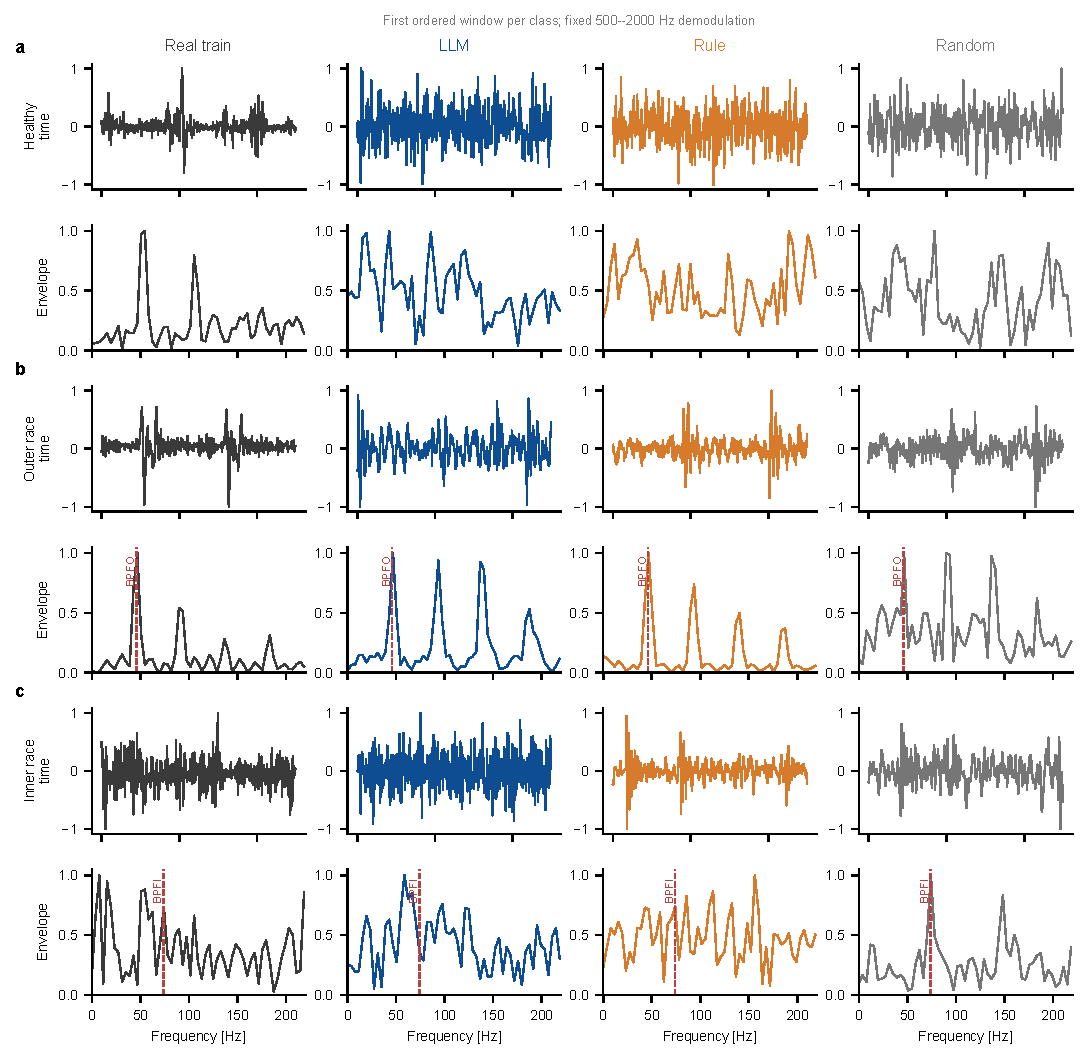
\includegraphics[width=\textwidth]{figs/waveforms.pdf}
  \caption{PU waveform and envelope-spectrum comparison. Rows are healthy,
  outer-race, and inner-race classes; columns compare real training, LLM,
  rule, and random open-loop windows. All envelope spectra use the same fixed
  500--2000 Hz demodulation band. Vertical markers denote the class-relevant
  kinematic frequency.}
  \label{fig:waves}
\end{figure*}

\begin{figure*}
  \centering
  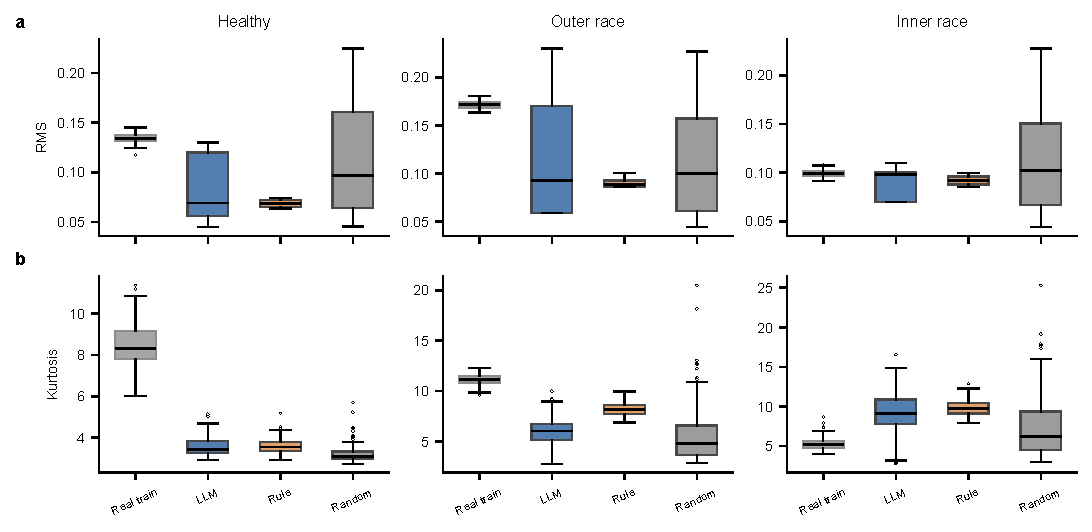
\includegraphics[width=\textwidth]{figs/boxplots.pdf}
  \caption{Class-conditional RMS and kurtosis distributions for the real PU
  training split and matched synthetic pools. Boxes show the frozen pool
  distributions; admission narrows unsupported statistical excursions without
  forcing equality to a single reference value.}
  \label{fig:boxplots}
\end{figure*}

\begin{figure*}
  \centering
  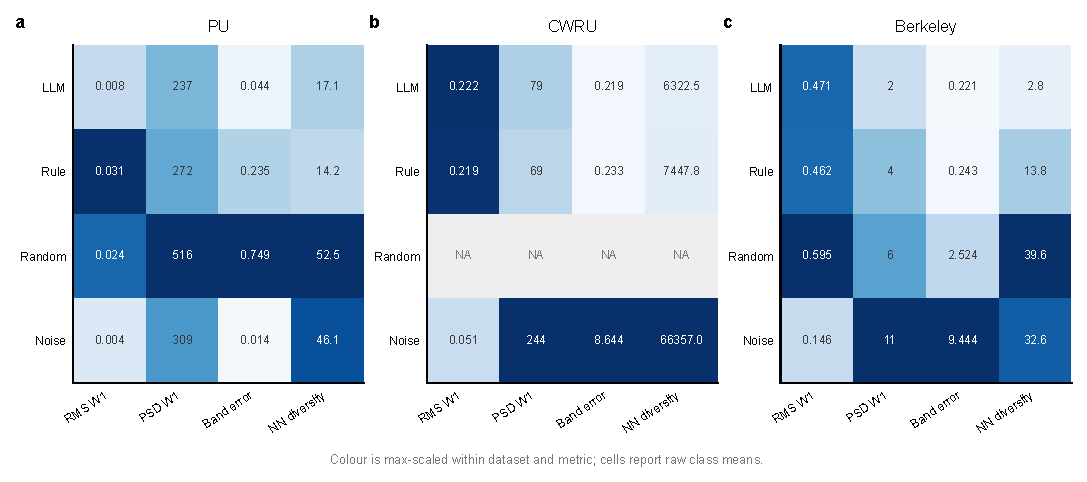
\includegraphics[width=\textwidth]{figs/metric_distances.pdf}
  \caption{Class-averaged physical diagnostics on PU, CWRU, and Berkeley.
  Cells contain raw RMS Wasserstein-1, PSD-CDF Wasserstein-1, relative
  band-energy error, and nearest-neighbour diversity values; colour is scaled
  within each dataset and metric only. NA denotes a pool that does not exist in
  the frozen archive, not an imputed value. Diversity has no universally
  optimal direction.}
  \label{fig:distances}
\end{figure*}

Table~\ref{tab:physics} gives the PU class averages. LLM recipes have lower
PSD distance and band-energy error than rule and random open-loop, and lower
RMS distance than those two recipe sources. Noise augmentation is closest in
RMS and band energy because it perturbs real windows directly, but it does not
provide a new recipe mechanism. Nearest-neighbour distance confirms that the
LLM pool is not a duplicate of its closest real reference under the frozen
feature metric; its value must be interpreted jointly with fidelity because
arbitrarily large distance can indicate unrealistic samples.

% Generated by breeze/scripts/build_paper_tables.py; do not edit.
\begin{table}[t]
\centering
\caption{Class-averaged PU physical diagnostics for fixed 150-window/class pools. Distances and errors are reference-relative diagnostics, not a downstream ranking; diversity has no preferred direction.}
\label{tab:physics}
\small
\begin{tabular}{lrrrr}
\toprule
pool & RMS W1 & PSD W1 & band-energy error & NN diversity \\
\midrule
llm & 0.008 & 236.9 & 0.044 & 17.10 \\
rule & 0.031 & 271.6 & 0.235 & 14.20 \\
random\_open\_loop & 0.024 & 516.1 & 0.749 & 52.50 \\
noise\_aug & 0.004 & 309.1 & 0.014 & 46.09 \\
\bottomrule
\end{tabular}
\end{table}


These diagnostics reduce, but cannot eliminate, circular validation. The
prompt, renderer, and verifier all encode bearing quantities, so passing the
same quantities is necessary rather than sufficient evidence of real-world
physics. The external downstream tests, rule/random controls, train/test
separation, and failed cross-condition experiments are therefore essential.

\subsection{Admission, slot-to-window accounting, and failure reasons}

Figure~\ref{fig:acceptance} resolves the slot/window ambiguity. PU requests
\BreezeProposalSlotsPerClass{} proposal slots per class. Panel (a) shows how many round candidates were
archived for each slot; panel (b) separates proposal slots, admitted slots, and
kept rendered windows; panel (c) compares verifier admission by recipe source.
At $K=3$, the archived LLM process admits \BreezeHealthyAdmissionRate\%,
\BreezeORAdmissionRate\%, and \BreezeIRAdmissionRate\% of
healthy/OR/IR slots. A random-recipe-plus-verifier audit admits no slot and
cannot form a balanced downstream pool. The rule source is class-dependent,
which explains why a fixed rule is a meaningful but incomplete substitute for
LLM proposal.

\begin{figure*}
  \centering
  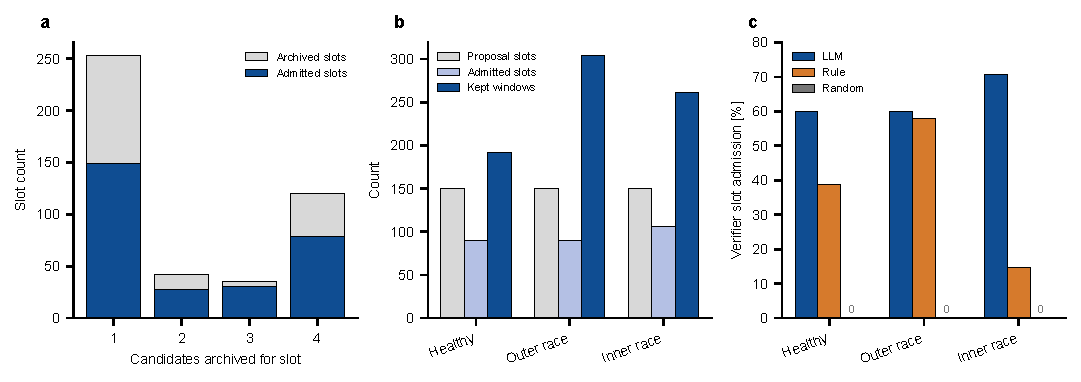
\includegraphics[width=\textwidth]{figs/acceptance_k.pdf}
  \caption{PU proposal accounting. (a) Number of archived candidates per
  proposal slot. (b) One-to-many mapping from
  \BreezeProposalSlotsPerClass{} class slots to admitted slots
  and diversity-kept windows. (c) Verifier slot-admission rates for LLM, rule,
  and random recipes. Random open-loop remains a downstream control; random
  recipes subjected to the verifier produce no balanced admitted pool.}
  \label{fig:acceptance}
\end{figure*}

Figure~\ref{fig:failreasons} reports non-exclusive terminal gate failures.
Random recipes fail statistical and spectral gates at much higher rates than
cached LLM recipes. Healthy LLM candidates are most often rejected for
unsupported envelope evidence, whereas fault candidates more often violate
the robust statistical domain. Because a slot may fail several gates,
percentages are not additive. This report is also the feedback payload: the
next round receives the measured violation rather than a generic ``try again''
instruction.

\begin{figure*}
  \centering
  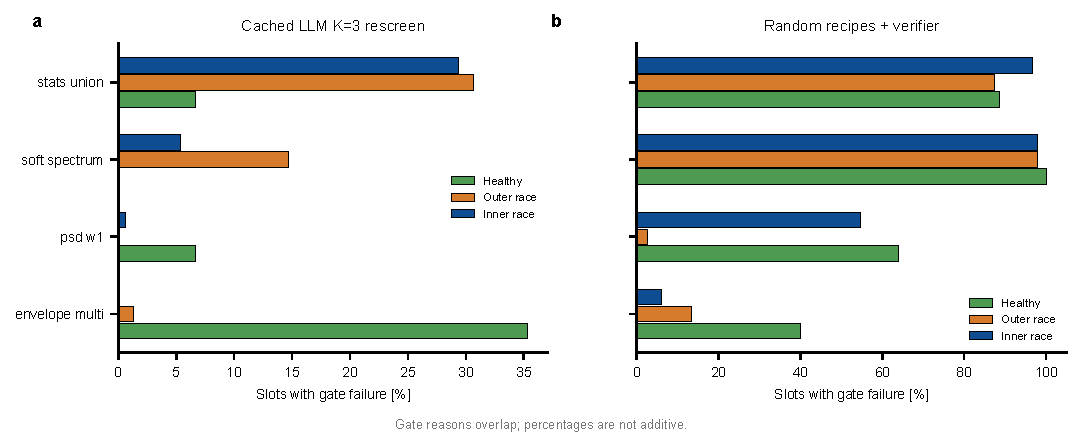
\includegraphics[width=\textwidth]{figs/failure_reasons.pdf}
  \caption{Non-exclusive PU gate-failure rates by class and recipe source.
  (a) Cached LLM $K=3$ rescreen. (b) Random recipes passed through the same
  verifier. Statistics, soft-spectrum, PSD-W1, and multi-band envelope failures
  are computed from frozen slot reports.}
  \label{fig:failreasons}
\end{figure*}

\section{Cross-condition evidence and negative results}
\label{sec:boundaries}

\subsection{CWRU success does not generalize to PU LOCO}

Figure~\ref{fig:cross} places the positive CWRU source-load0 transfer result
beside the PU LOCO audit. PU v1 fails
\BreezePULOCOVOneFailures/\BreezePULOCORegisteredTests{} registered cells and
v2 fails \BreezePULOCOVTwoFailures/\BreezePULOCORegisteredTests{}. Failures cluster
by held-out condition and persist across Accuracy/Macro-F1 and shot counts.
Thus the load0-derived recipe representation transfers to the tested CWRU
loads 1--3, but it does not reliably extrapolate PU condition-dependent
morphology.

\begin{figure*}
  \centering
  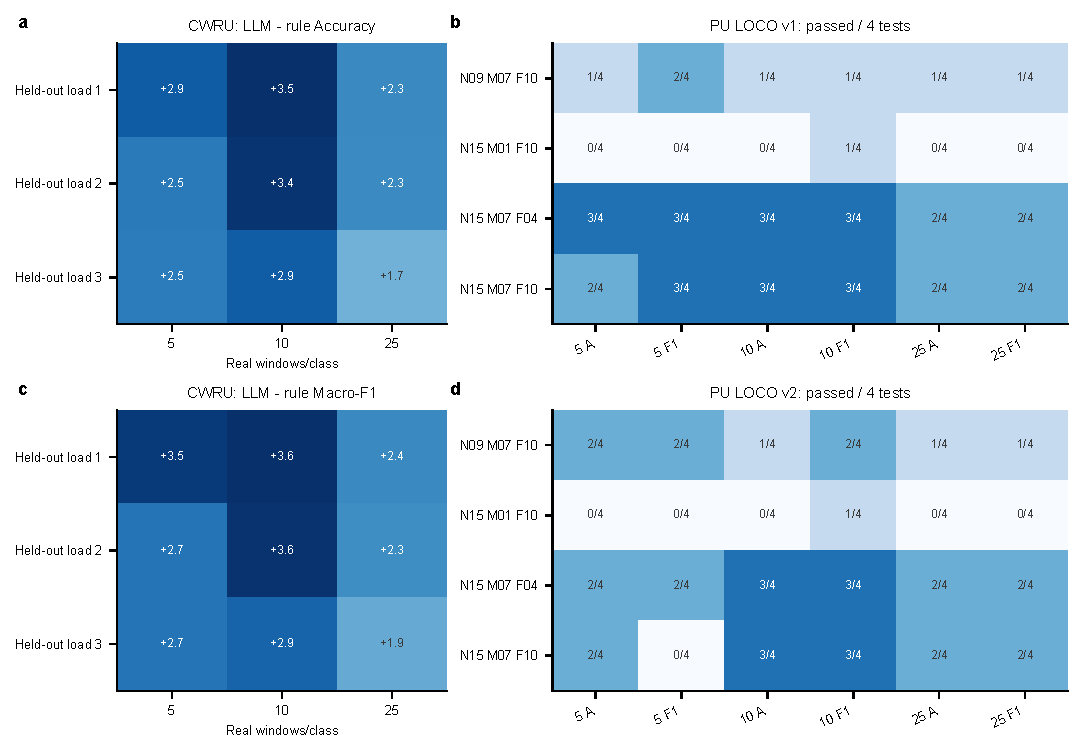
\includegraphics[width=\textwidth]{figs/cross_condition_heatmap.pdf}
  \caption{Cross-condition evidence. (a,c) CWRU LLM--rule Accuracy and
  Macro-F1 deltas when load0-derived pools are evaluated on held-out loads
  1--3. The archived held-out-load0 fold is excluded for target-load
  provenance. (b,d) Number of passed PU LOCO tests out of four registered
  comparisons in each condition--shot--metric cell for v1 and v2.}
  \label{fig:cross}
\end{figure*}

The PU investigation followed six predeclared stages
(Fig.~\ref{fig:failurechain}). v1 exposed kinematic mismatch. v2 corrected
frequency handling but did not restore downstream success. v3 attempted
train-condition morphology mapping and could not form an admissible balanced
pool. v4 tested two train-only candidate-pool strategies; neither passed its
admission requirements. v5 admitted wrong-label/noise controls, showing that
the candidate criterion was not discriminative. v6 evaluated source-only
cyclostationary coherence; the score failed to separate all four held-out
targets, so no formal downstream test was authorized. Only v1 and v2 are
formal held-out evaluations. v3--v6 are development/admission stops, and are
not re-labelled as hidden test results.

\begin{figure*}
  \centering
  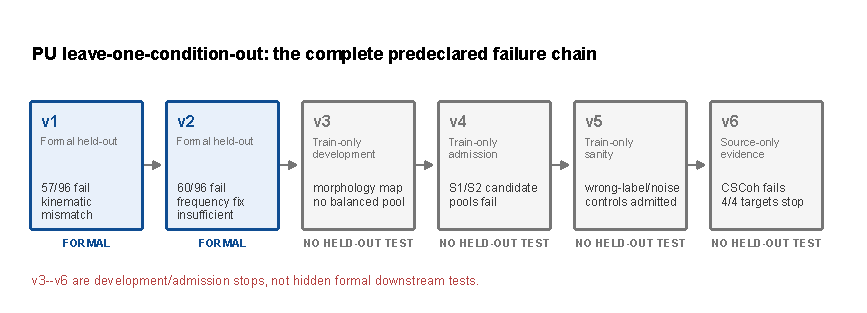
\includegraphics[width=\textwidth]{figs/failure_case.pdf}
  \caption{Complete PU LOCO failure chain. v1 and v2 are formal held-out
  evaluations; v3--v6 stop at train-only morphology, admission, sanity, or
  source-only evidence gates. The sequence prevents unsuccessful development
  stages from being reported as completed cross-condition tests.}
  \label{fig:failurechain}
\end{figure*}

\subsection{Milling boundaries}

The private machine-tool dataset used in earlier drafts is removed from the
core evidence because its speed, geometry, file-to-operation manifest, and
audited physical label mapping are incomplete. It cannot support a public or
reproducible portability claim.

UMich milling is also not described as ``unlearnable.'' In the available
protocol, experimental condition and process metadata are confounded with wear
labels. A classifier can therefore exploit condition identity instead of wear,
and the current files do not permit those effects to be disentangled. A valid
formal test requires additional repeated conditions or a revised acquisition
design. MU-TCM v3 stops earlier: only
\BreezeMUTCMPassedTests/\BreezeMUTCMRegisteredTests{} predeclared train-only inner-
validation comparisons pass, so neither preregistration nor a formal held-out
test was executed. Neither dataset contributes a positive result.

\section{Discussion}
\label{sec:discussion}

\subsection{What the experiments establish}

Three conclusions are supported. First, the language proposal is not
replaceable by arbitrary recipe sampling in the PU protocol: random recipes
cannot form a balanced verified pool, and random open-loop augmentation is
substantially weaker downstream. Second, the LLM adds value beyond a fixed
rule recipe in all registered PU cells and all provenance-valid CWRU families. Third,
that advantage is not universal: Berkeley LLM and rule recipes converge at ten
shots, and PU LOCO fails despite repeated representation changes.

The contribution is therefore neither a general-purpose physical simulator nor
a new trained generative model. It is a train-calibrated control layer around a
structured black-box proposal source. This operating point is useful when a
new target generator cannot be trained, when rejection records are required,
or when engineers need to inspect exactly why a sample entered the pool.

\subsection{Physical verification versus physical truth}

The verifier measures observables selected by bearing and signal-processing
theory. Those observables are incomplete. A candidate can satisfy RMS, PSD,
and envelope gates while missing load-path, transfer-function, non-stationary,
or degradation mechanisms. Conversely, a rare but real sample can fall outside
a finite training boundary. For this reason, \breeze\ reports class-wise
distances, downstream tests, and negative transfer results alongside gate
pass rates. A pass should be read as ``admissible under the declared training-
calibrated gates,'' not as a proof of membership in the full real distribution.

The architecture also creates a circularity risk: the renderer and verifier
share some kinematic quantities. Matched rule and random sources partially
break that circle because all sources see the same renderer and physical
checks, yet only the LLM source consistently produces useful admitted pools.
Further reduction of this risk requires external expert scoring, independent
physical observables not present in the prompt, and new condition-disjoint
datasets.

\subsection{Reproducibility and remaining blockers}

The repository stores split manifests, prompts, recipe JSON, local renderer
seeds, waveform hashes, per-gate reports, pool manifests, seed-level classifier
rows, registered tests, and table-generation assertions. Long-running
pipelines are append-only or checkpoint-resumable. Every number in the paper
is generated from frozen CSV/NPZ artifacts; missing pools are displayed as NA
rather than substituted.

Two limitations remain material. First, the original PU provider version and
provider-side sampling seed were not captured, so exact replay begins from the
archived recipes rather than from the LLM response. Second, completed formal
TimeGAN/DDPM and additional diagnostic-backbone comparisons are not available.
Accordingly, no state-of-the-art or universal classifier claim is made. Future
work should complete those matched baselines, repeat the protocol with at least
one non-CNN diagnostic backbone, and preregister a new PU cross-condition
representation before accessing held-out outcomes.

\section{Conclusion}
\label{sec:conclusion}

\breeze\ separates LLM recipe proposal, fixed seeded rendering, train-
calibrated physical admission, and downstream diagnosis. Under frozen public
protocols, LLM recipes outperform matched rule and random/non-structured
controls on PU and CWRU and provide a qualified lower-shot benefit on Berkeley
milling. Physical diagnostics and gate reports make the admitted pools
inspectable, while the complete PU LOCO, UMich, and MU-TCM failures define the
current boundary. The evidence supports a training-free, physics-verified
admission workflow for few-shot condition monitoring. It does not support
zero-data diagnosis, formal physical guarantees, or universal superiority over
trained generative models.

\section*{Data and code availability}

PU and CWRU are public benchmark datasets, and Berkeley milling is available
through the NASA prognostics repository subject to its terms. The manuscript
tables are generated by \texttt{scripts/build\_paper\_tables.py}. Numerical
sources, availability records, and permitted claim wording are enumerated in
\texttt{analysis/evidence\_ledger.md} and
\texttt{analysis/claim\_evidence\_map.md}. Release artifacts include gate
thresholds, per-sample pass/fail records, pool manifests, split audits, and
seed-level downstream outputs. API credentials and raw third-party datasets
are not distributed.

\section*{Declaration of competing interest}

The authors declare that they have no known competing financial interests or
personal relationships that could have appeared to influence the work
reported in this paper.

\section*{Declaration of generative AI and AI-assisted technologies}

During preparation of this work, the authors used OpenAI Codex for code
inspection, experiment orchestration, figure and table assembly, and language
editing. The authors reviewed the evidence, verified the reported results, and
take responsibility for the manuscript.

\bibliographystyle{cas-model2-names}
\bibliography{references}

\end{document}
